\documentclass[a4paper,12pt]{article}
\usepackage[T2A]{fontenc}
\usepackage[utf8]{inputenc}
\usepackage[russian]{babel}
\usepackage{geometry}
\usepackage{hyperref}
\usepackage{enumitem}
\usepackage{graphicx}
\usepackage{tikz}

\geometry{a4paper, total={170mm,257mm}, left=20mm, top=20mm}

\title{\textbf{Rust Team Lead}}
\author{Алексей Леонидович Беляков}
\date{\today}

\newcommand{\avatar}{%
    \begin{center}
        \begin{tikzpicture}
            \clip (0,0) circle (1.5cm);
            \node at (0,0) {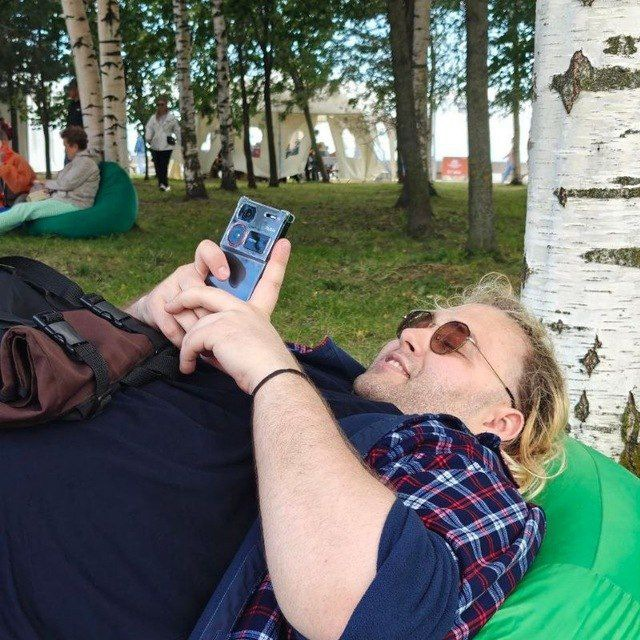
\includegraphics[width=3cm,height=3cm]{../../content/avatar.jpg}};
        \end{tikzpicture}
    \end{center}}

\begin{document}

\maketitle

\avatar

\begin{center}
    \begin{tabular}{rl}
        \textbf{Телефон:} & +7 (911) 261-70-72 \\
        \textbf{Telegram:} & \href{https://leqqrm.t.me}{leqqrm.t.me} \\
        \textbf{Почта:} & \href{mailto:qqrm@vivaldi.net}{qqrm@vivaldi.net} \\
        \textbf{GitHub:} & \href{https://github.com/qqrm}{github.com/qqrm} \\
        \textbf{Docs:} & \href{https://qqrm.github.io/CV/}{qqrm.github.io/CV} \\
    \end{tabular}
\end{center}

\vspace{5mm}

\section*{Языки}
\begin{itemize}[leftmargin=15pt]
    \item Русский (родной)
    \item Английский (B2 — продвинутый уровень)
\end{itemize}

\section*{Цель}
Ведущий Rust-разработчик с почти 10-летним опытом в разработке программного обеспечения и системной архитектуре. Ориентирован на создание высокопроизводительных, отказоустойчивых систем и работу с командами для достижения заметных результатов. Ищу возможности для применения глубоких технических знаний, лидерских навыков и лучших практик микросервисной архитектуры, чтобы формировать эффективные коллективы разработчиков, совершенствовать процессы и помогать бизнесу достигать целей в современных технологических проектах.

\section*{Опыт работы}

\subsection*{Rust Team Lead @ Inline Group}
\quad март 2024 – настоящее время, ~1 год
\begin{itemize}[leftmargin=15pt]
    \item Руководил бэкенд-командой из 12 человек (в рамках проекта численностью 40+ человек) в инициативе по импортозамещению и миграции бизнес-процессов с SAP на собственную микросервисную архитектуру на Rust.
    \item Проектировал и развивал микросервисы на базе \textbf{Actix Web}, \textbf{RabbitMQ}, \textbf{PostgreSQL} и других технологий, обеспечивая высокую производительность и надёжность.
    \item Внедрил и контролировал соблюдение Agile-практик (Scrum, спринты, ежедневные стендапы, ретроспективы), что позволило увеличить скорость разработки примерно на \(\sim 20\%\) и снизить объём доработок.
    \item Определил требования к инфраструктуре (конвейеры CI/CD, тестовые среды) и взаимодействовал с командой DevOps для оптимизации развёртывания в корпоративном контуре.
    \item Организовал процесс найма и онбординга: расширил бэкенд-команду с 5 до 12 человек, сократив среднее время адаптации примерно на \(\sim 30\%\).
    \item Реализовал собственный Cargo-регистр с учётом жёстких требований информационной безопасности, а также интегрировал статический анализ кода (\textit{Clippy}, \textit{cargo-audit}, \textit{SonarQube}) в сборочный конвейер.
    \item Отвечал за принятие архитектурных решений, код-ревью и оптимизацию производительности; сократил бэклог багов примерно на \(\sim 30\%\) благодаря ужесточению QA-процессов.
    \item Сотрудничал с бизнес-аналитиками и ключевыми заказчиками для преобразования требований SAP в микросервисные решения, что снизило время вывода новых фич на рынок примерно на \(\sim 25\%\).
\end{itemize}

\textbf{Достижения:}
\begin{itemize}[leftmargin=15pt]
    \item Повысил продуктивность спринтов на \(\sim 15\%\) благодаря внедрению асинхронного подхода и персонализированному планированию.
    \item Улучшил предсказуемость спринтов на \(\sim 25\%\) за счёт более точных оценок и качественного ведения бэклога.
    \item Внёс ясность в систему отчётности и формирование дорожных карт для стейкхолдеров, наладив эффективную кросс-командную коммуникацию и согласование приоритетов.
\end{itemize}

\textbf{Технологии}: Rust, Actix Web, RabbitMQ, PostgreSQL, Docker, GitLab CI/CD, Odoo, Clippy, cargo-audit, SonarQube

\vspace{3mm}

\subsection*{Lead Rust Developer @ YADRO}
\quad март 2023 – март 2024, 1 год
\begin{itemize}[leftmargin=15pt]
    \item Улучшал архитектуру аппаратно-программного комплекса для решения резервного копирования на базе дедупликации.
    \item Изучал способы оптимизации \textbf{RocksDB} и повышения производительности NVMe-дисков.
    \item Реализовал структуры данных для эффективного хранения хэшей и метахэшей.
    \item Исправлял ошибки и совершенствовал модули сжатия и дедупликации.
    \item Проводил код-ревью и читал внутренние лекции по Rust, помогая бывшим C++-разработчикам перейти на идиоматичный Rust, что сократило время онбординга примерно на \(\sim 30\%\).
\end{itemize}

\textbf{Технологии}: Rust, Tokio, Protocol Buffers, Serde, RocksDB, Git

\vspace{3mm}

\subsection*{Senior Rust/Python Developer (частичная занятость) @ Ultima-bi}
\quad ноябрь 2022 – март 2023, 5 месяцев
\begin{itemize}[leftmargin=15pt]
    \item Разработал \textbf{Python}-обёртки и систему кеширования для инструмента Data Science на базе \textbf{Polars}, обеспечив бесшовную интеграцию Rust \(\leftrightarrow\) Python.
    \item Использовал \textbf{PyO3} для ускорения критически важных участков кода, добившись примерно \(\sim 25\%\) прироста скорости обработки данных.
    \item Спроектировал автоматизированные тесты для повышения надёжности и удобства сопровождения гибридного решения на Python и Rust.
\end{itemize}

\textbf{Технологии}: Rust, Python3, PyO3, Git

\vspace{3mm}

\subsection*{Rust Team Lead @ Solcery}
\quad март 2022 – март 2023, 1 год
\begin{itemize}[leftmargin=15pt]
    \item Руководил командой из 4 Rust-разработчиков при создании блокчейн-базы данных на \textbf{Solana}, ориентированной на DAO и каркас для карточных игр.
    \item Проектировал и внедрял низкоуровневые структуры хранения данных, версиирование и миграции таблиц, снизив сложность кода на \(\sim 20\%\).
    \item Сформировал требования на основе пользовательских историй, совмещая технические и бизнес-аспекты.
    \item Координировал спринты, распределял задачи, следил за сроками и своевременным релизом ключевых фич.
    \item Проводил код-ревью, что позволило сократить количество ошибок на продакшене примерно на \(\sim 30\%\) благодаря раннему выявлению проблем.
\end{itemize}

\textbf{Достижения:}
\begin{itemize}[leftmargin=15pt]
    \item Упростил рабочий процесс разработки на Rust, сократив среднее время код-ревью на 40\%.
    \item Ввёл передовые практики версионирования и миграций, обеспечив бесшовное использование DAO-подхода в игровых фреймворках.
\end{itemize}

\textbf{Технологии}: Rust, Solana Test Validator, Git, GitHub

\vspace{3mm}

\subsection*{Senior Rust Developer @ Kaspersky Lab \quad (май 2021 – март 2022, 11 месяцев)}
\begin{itemize}[leftmargin=15pt]
    \item Поддерживал и развивал блокчейн-сервис голосования на базе \textbf{Exonum}, добавляя функциональность голосования с учётом «веса» участников.
    \item Расширил покрытие интеграционными и модульными тестами примерно до \(\sim 75\%\), укрепив общее качество кода.
    \item Участвовал в миграции экосистемы на решения Microsoft, совершенствуя CI/CD для более быстрых развёртываний.
\end{itemize}

\textbf{Достижения:}
\begin{itemize}[leftmargin=15pt]
    \item Снизил проблемы на этапе пост-релиза примерно на \(\sim 25\%\) за счёт более плотного покрытия тестами и надёжного конвейера CI.
    \item Рефакторил кодовую базу для упрощения поддержки и добавления новых функций.
\end{itemize}

\textbf{Технологии}: Rust, Exonum, Protocol Buffers, Serde, Git

\vspace{3mm}

\subsection*{Rust Developer @ Kryptonite}
\quad май 2020 – май 2021, 1 год 1 месяц
\begin{itemize}[leftmargin=15pt]
    \item Перенёс систему обработки голосовых вызовов со \textbf{Scala} на \textbf{Rust}, повысив производительность и снизив расход памяти.
    \item Реализовал нормализацию записей разговоров и анализ на основе эмбеддингов для высокоточной индексации.
    \item Разработал модули синхронизации многоканальных диалогов, повысив целостность данных.
    \item Создал комплексные наборы юнит-тестов для проверки новых функций и стабильности системы.
\end{itemize}

\textbf{Достижения:}
\begin{itemize}[leftmargin=15pt]
    \item Добился \(\sim 20\%\) прироста производительности относительно версии на Scala, ускорив анализ звонков.
    \item Уменьшил объём использования памяти примерно на \(\sim 25\%\) за счёт оптимизации конкурентных паттернов в Rust.
\end{itemize}

\textbf{Технологии}: Rust, PostgreSQL, nalgebra, Serde, Protocol Buffers, Tokio, Git

\vspace{3mm}

\subsection*{Senior C++/Go Developer @ B2Broker \quad (ноябрь 2018 – март 2020, 1 год 6 месяцев)}
\begin{itemize}[leftmargin=15pt]
    \item Разрабатывал финансовое ПО с использованием \textbf{MT4/MT5} API, в том числе трейд-копиры на C++ и Go.
    \item Создал «Multi Account Manager» для гибкого распределения средств и расчёта вознаграждений, повышая операционную эффективность примерно на \(\sim 15\%\).
    \item Проектировал микросервисы на C++ и Go для нормализации и доставки данных из MT4/MT5 к виджетам, обеспечивая обработку в реальном времени.
    \item Реализовал сборщики данных для статистического анализа, давая брокерам более глубокие инсайты.
\end{itemize}

\textbf{Технологии}: MSVC, CMake, Protocol Buffers, gRPC, NATS, YAML, PostgreSQL, Vcpkg, Git

\vspace{3mm}

\subsection*{Middle → Senior C++ Developer @ ASCON \quad (май 2016 – ноябрь 2018, 2 года 7 месяцев)}
\begin{itemize}[leftmargin=15pt]
    \item Участвовал в разработке библиотек для архитектурного проектирования (KOMPAS), внедрив функцию «Change View Plane» для улучшения 3D-моделирования.
    \item Создал фреймворк автоматизированного тестирования (C++/Python), что сократило ручные проверки примерно на \(\sim 30\%\).
    \item Принимал участие в масштабном рефакторинге, перейдя на \textbf{C++17}.
    \item Внёс в процесс использования Git, Slack и интеграционных тестов, повысив эффективность командного взаимодействия.
\end{itemize}

\textbf{Технологии}: MSVC, C++, Boost, kompas-api, Python, Git, SVN, CMake

\vspace{3mm}

\subsection*{Middle C++ Developer @ Con Certeza \quad (март 2015 – апрель 2016, 1 год 2 месяца)}
\begin{itemize}[leftmargin=15pt]
    \item Разработал сниффер и парсер сигнального трафика (полный стек SS7) в рамках системы СОРМ для МТС.
    \item Написал парсеры для \textbf{INAP}, \textbf{RANAP}, \textbf{MAP}, \textbf{TCAP}, \textbf{CAP}, \textbf{MTP3}, \textbf{MTP2}, \textbf{SCCP}, \textbf{SIP}.
    \item Создал модули для сбора информации из трафика (SMS, перемещения абонентов, телефонные вызовы) на базе RFC-протоколов.
    \item Разработал интеграционные тесты на Python для проверок реализованного функционала.
\end{itemize}

\textbf{Технологии}: Myri10GE API, libpcap, PF\_RING, C++11, Boost, Python

\vspace{3mm}

\subsection*{Middle C++/JS Developer @ LiveTex \quad (июль 2014 – март 2015, 7 месяцев)}
\begin{itemize}[leftmargin=15pt]
    \item Создал обёртки для \textbf{PostgreSQL} и \textbf{ZeroMQ} под Node.js, сократив задержки выполнения запросов примерно на \(\sim 10\%\).
\end{itemize}

\textbf{Технологии}: GCC, C++, Node.js, JavaScript

\vspace{3mm}

\subsection*{Junior C++ Developer @ Tools for Brokers \quad (ноябрь 2013 – июль 2014, 9 месяцев)}
\begin{itemize}[leftmargin=15pt]
    \item Выполнял разработку для платформ \textbf{MetaTrader 4} и \textbf{5}.
    \item Улучшал и отлаживал плагин для взаимных фондов (\textbf{UMAM}).
    \item Создал веб-приложение для управления сервером MT4, повысив эффективность администрирования примерно на \(\sim 15\%\).
\end{itemize}

\textbf{Технологии}: C++, Boost, C\#, JavaScript

\end{document}
